\documentclass[border=3pt]{standalone}
% Shared TikZ styles for the Ch. 3–8 diagrams (standalone PDFs); extends the Ch. 1 palette (s1_vs_llm_common.tex).
\usepackage[T1]{fontenc}
\usepackage{lmodern}
\usepackage[english]{babel}
\usepackage{amsmath,amssymb}
\usepackage{tikz}
\usetikzlibrary{shapes.geometric,shapes.misc,positioning,fit,arrows.meta,calc,backgrounds,decorations.pathreplacing,patterns}
\definecolor{ioFill}{HTML}{F1F0EC}\definecolor{ioLine}{HTML}{52514E}
\definecolor{modFill}{HTML}{E8F1FB}\definecolor{modLine}{HTML}{2A78D6}
\definecolor{decFill}{HTML}{ECE9F7}\definecolor{decLine}{HTML}{4A3AA7}
\definecolor{postFill}{HTML}{FFF6E0}\definecolor{postLine}{HTML}{EDA100}
\definecolor{okFill}{HTML}{EAF7F1}\definecolor{okLine}{HTML}{1BAF7A}
\definecolor{badFill}{HTML}{FDECEC}\definecolor{badLine}{HTML}{E34948}
\definecolor{nmFill}{HTML}{EFEAF8}\definecolor{nmLine}{HTML}{4A3AA7}
\definecolor{loopRed}{HTML}{E34948}\definecolor{clusterLine}{HTML}{9A9890}\definecolor{ink2}{HTML}{52514E}
\definecolor{orangeA}{HTML}{EB6834}
\tikzset{
  every node/.style={font=\small, align=center},
  io/.style={trapezium, trapezium left angle=72, trapezium right angle=108, trapezium stretches body,
             draw=ioLine, fill=ioFill, thick, inner sep=3pt, minimum height=2.4em},
  model/.style={rectangle, draw=modLine, fill=modFill, very thick, inner sep=4pt, minimum height=2.4em, text width=#1},
  model/.default=3.6cm,
  post/.style={rectangle, draw=postLine, fill=postFill, very thick, inner sep=4pt, minimum height=2.2em, text width=#1},
  post/.default=3.6cm,
  data/.style={cylinder, shape border rotate=90, aspect=0.18, draw=okLine, fill=okFill, very thick, inner sep=3pt, minimum height=2.6em, text width=#1},
  data/.default=2.4cm,
  decision/.style={diamond, aspect=2.1, draw=decLine, fill=decFill, very thick, inner sep=1pt},
  outcome/.style={rounded rectangle, draw=#1, thick, inner sep=4pt, minimum height=2em},
  arrow/.style={-{Latex[length=2mm]}, thick, ioLine},
  dashedarrow/.style={-{Latex[length=2mm]}, thick, ioLine, dashed},
  loop/.style={-{Latex[length=2.4mm]}, line width=1.4pt, loopRed},
  cluster/.style={draw=clusterLine, dashed, rounded corners=3pt, inner sep=7pt},
  clusterlabel/.style={font=\small\bfseries, text=ioLine},
  note/.style={font=\footnotesize, text=ink2},
  tok/.style={rectangle, draw=ioLine, fill=ioFill, thin, inner sep=2pt, minimum height=1.6em, font=\footnotesize},
  vmark/.style={rectangle, draw=orangeA, fill=postFill, thick, inner sep=2pt, minimum height=1.6em, font=\footnotesize\ttfamily},
}

\begin{document}
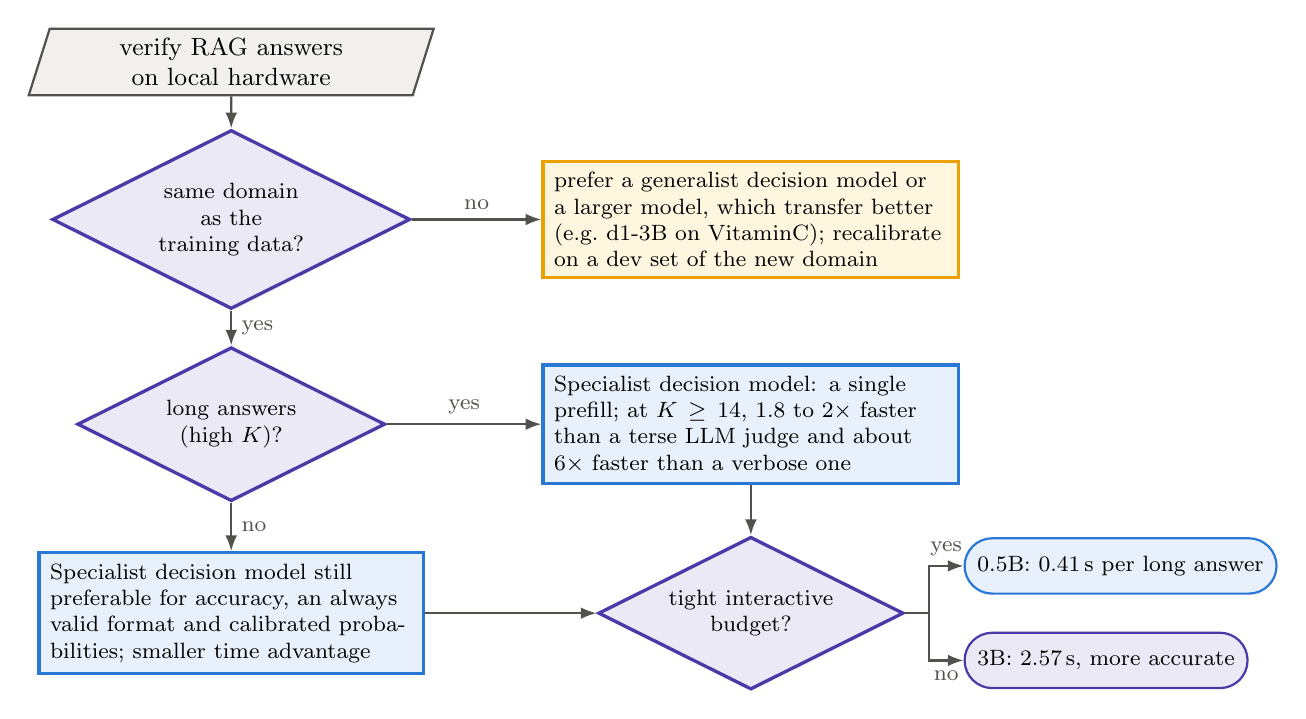
\begin{tikzpicture}
  \node[io, text width=4.4cm] (s) at (0,0) {verify RAG answers\\on local hardware};
  \node[decision, font=\footnotesize, text width=2.5cm, aspect=2.0] (d1) at (0,-2.0) {same domain\\as the\\training data?};
  \node[post=5.0cm, font=\footnotesize, align=left] (gen) at (6.6,-2.0) {prefer a generalist decision model or a larger model, which transfer better (e.g.\ d1-3B on VitaminC); recalibrate on a dev set of the new domain};
  \node[decision, font=\footnotesize, text width=2.5cm, aspect=2.0] (d2) at (0,-4.6) {long answers\\(high $K$)?};
  \node[model=5.0cm, font=\footnotesize, align=left] (long) at (6.6,-4.6) {Specialist decision model: a single prefill; at $K \geq 14$, $1.8$ to $2\times$ faster than a terse LLM judge and about $6\times$ faster than a verbose one};
  \node[model=4.6cm, font=\footnotesize, align=left] (short) at (0,-7.0) {Specialist decision model still preferable for accuracy, an always valid format and calibrated probabilities; smaller time advantage};
  \node[decision, font=\footnotesize, text width=2.5cm, aspect=2.0] (d3) at (6.6,-7.0) {tight interactive\\budget?};
  \node[outcome=modLine, fill=modFill, font=\footnotesize, anchor=west] (s05) at (9.3,-6.4) {0.5B: 0.41\,s per long answer};
  \node[outcome=decLine, fill=decFill, font=\footnotesize, anchor=west] (s3) at (9.3,-7.6) {3B: 2.57\,s, more accurate};
  \draw[arrow] (s) -- (d1);
  \draw[arrow] (d1) -- node[above, font=\footnotesize] {no} (gen);
  \draw[arrow] (d1) -- node[right, font=\footnotesize] {yes} (d2);
  \draw[arrow] (d2) -- node[above, font=\footnotesize] {yes} (long);
  \draw[arrow] (d2) -- node[right, font=\footnotesize] {no} (short);
  \draw[arrow] (long) -- (d3);
  \draw[arrow] (short) -- (d3);
  \draw[arrow] (d3.east) -- ++(3mm,0) |- node[pos=0.75, above, font=\footnotesize] {yes} (s05.west);
  \draw[arrow] (d3.east) -- ++(3mm,0) |- node[pos=0.75, below, font=\footnotesize] {no} (s3.west);
\end{tikzpicture}
\end{document}
